\documentclass[11pt]{article}
\usepackage[margin=0.85in]{geometry}
\usepackage[T1]{fontenc}
\usepackage{lmodern}
\usepackage{graphicx}
\usepackage{booktabs}
\usepackage{array}
\usepackage{xcolor}
\usepackage{hyperref}
\usepackage{pdfpages}
\usepackage{caption}
\usepackage{float}
\usepackage{microtype}
\hypersetup{colorlinks=true,linkcolor=blue!55!black,urlcolor=blue!55!black,citecolor=blue!55!black}
\graphicspath{{../images/}}
\setlength{\parskip}{0.45em}
\setlength{\parindent}{0pt}
\title{\textbf{Reading Chase Pressure at the Six-Over Mark}\\[0.3em]
\large DAS732 Programming Assignment 3: Visual Analytics Workflow}
\author{Team 3\\\small IIIT Bangalore, Term 1 (2026--27)\\[0.5em]
\small Team members, listed in A2 disclosures (confirm A3 roster):\\
K V Shashank Pai (BT2024250); Adithya Kommuri (BT2024246);\\
Nishanth Karamsetty (BT2024094)}
\date{November 2026}
\begin{document}
\maketitle

\begin{abstract}
This project studies whether the score and wickets after six completed overs explain eventual IPL chase success, and whether the target-relative required run rate adds useful context. From 1,194 eligible match states, we compare a raw-state view and model with a target-aware second iteration. A season-block bootstrap estimates the difference in win rates between the lowest and highest required-rate quartiles as 70.7\% (95\% interval 65.0\% to 76.3\%). On a later-date holdout, the raw-state logistic model has ROC--AUC 0.729 and the target-aware model has ROC--AUC 0.890. The project treats these as descriptive and predictive patterns, not causal effects.
\end{abstract}

\section{Introduction and problem statement}
The A1 IPL story explored scoring trends, team and player profiles, bowling, toss decisions, and venues. This A3 analysis narrows the focus to one moment: the end of six legal overs in a second innings. The research question is: \textit{How do runs and wickets at this checkpoint relate to chase success, and what additional information is contained in the required scoring rate implied by the first-innings target?}

This question is useful for studying how raw progress depends on the task still remaining. It does not assert that pressure causes a team to win or lose. The main contribution beyond A1 is a reproducible match-state table, unsupervised state grouping, a leakage-aware supervised model, and an inference-triggered transformation followed by a second visual iteration.

\section{Dataset and preparation}
The primary data are the A1 IPL match and delivery tables: 1,243 matches and 295,732 ball-level rows over 19 season labels from 2008-04-18 to 2026-05-31. The A1 report and its 15 visualizations are included in Appendix A for context; their old figures and conclusions are not presented as new A3 analyses. A2's gridMET meteorological data were inspected but not added because they do not materially support an IPL chase question.

The unit of analysis is one match's second-innings state after 36 legal balls in overs 0--5. Target equals first-innings total runs plus one. Chase success is whether the second-innings batting team matches the official winner. The pipeline retains all source delivery rows and excludes super-over events, ties, no-results, D/L matches, matches scheduled for fewer than seven overs, and innings with fewer than 36 legal balls in the first six overs. The final table contains 1,194 observations (649 successful chases and 545 unsuccessful chases). The filtering does not remove outliers for visual convenience.

\section{Visual analytics workflow}
The workflow follows Keim et al.'s visual analytics process: data, visualization, modeling, and knowledge formation interact through bidirectional flows, while self-loops represent refinement within a stage. Here, knowledge means an inference supported by the analysis. Figure~\ref{fig:workflow} shows both this cyclic view and its unrolled, end-to-end execution. The first pass moves from data through visualization and modeling to result visualization. Its inference is that raw six-over runs and wickets omit target context. This knowledge feeds back by adding runs remaining and required run rate to the dataset representation. The next pass analyzes and visualizes the transformed state, compares models on the same holdout, and records a final inference. The matches and outcomes stay fixed across the transformation.

\begin{figure}[H]
\centering
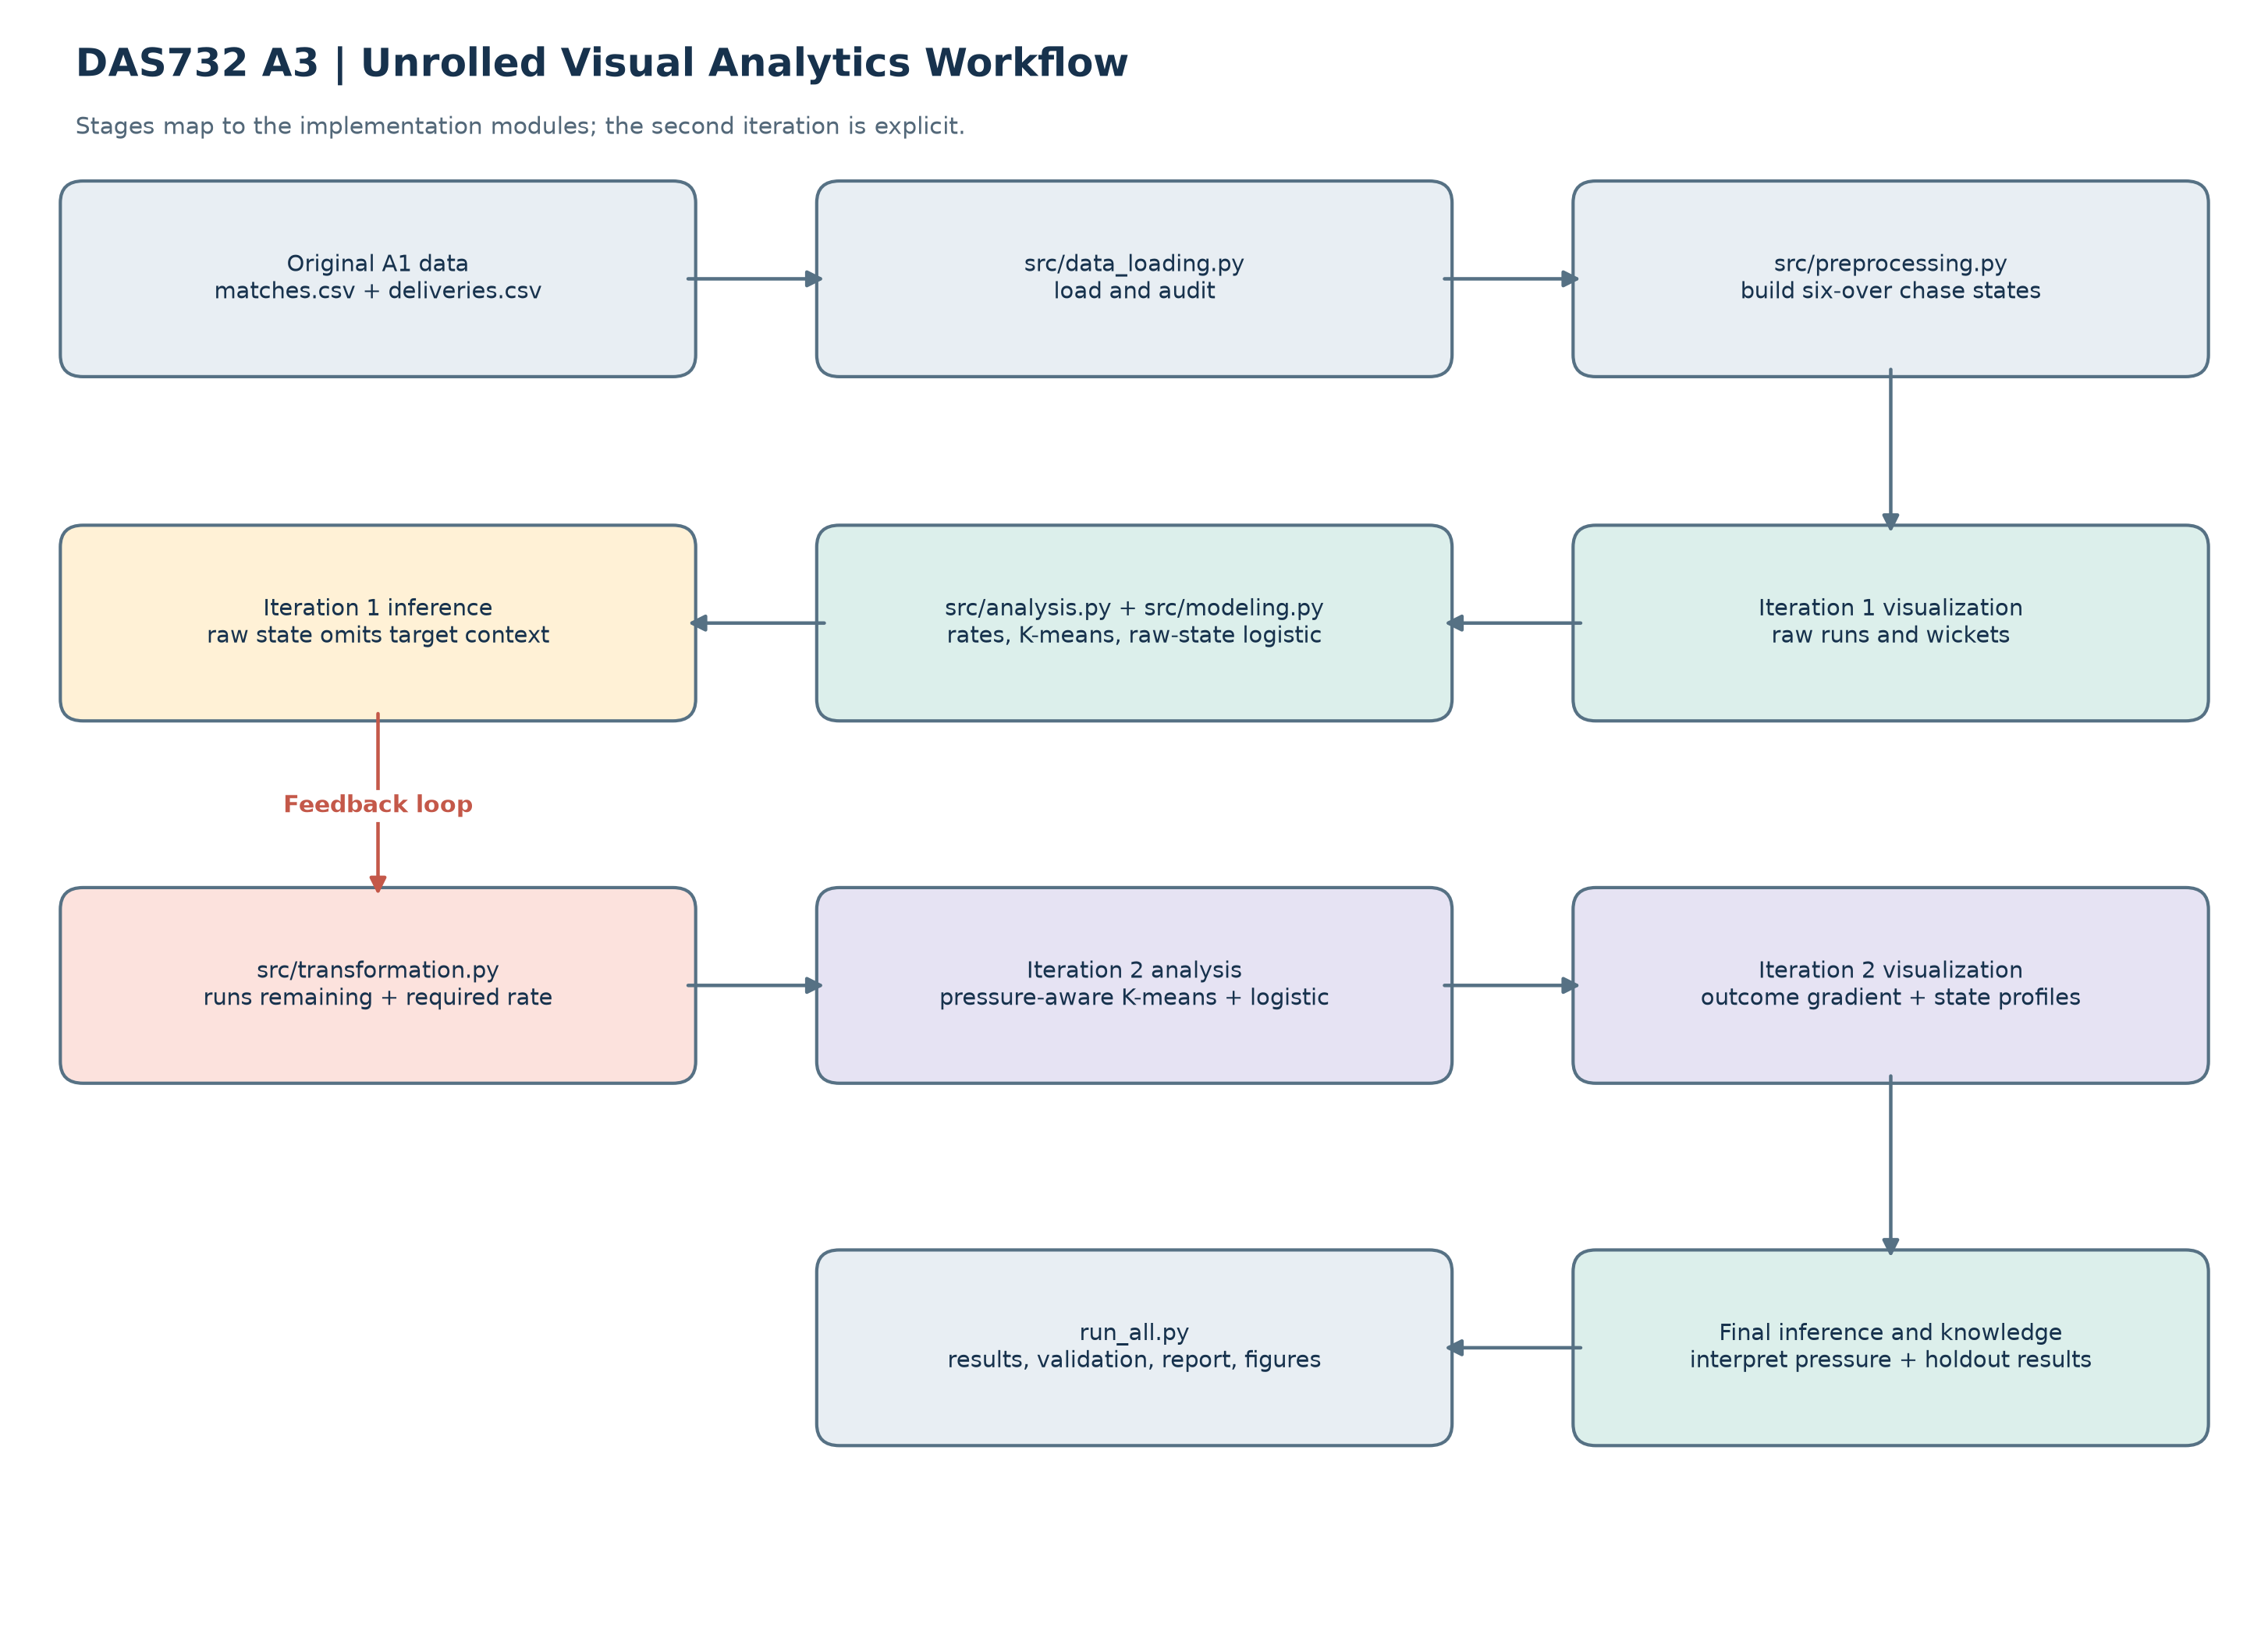
\includegraphics[width=0.94\linewidth]{workflow_diagram.png}
\caption{Cyclic and unrolled visual analytics workflow. The upper view shows bidirectional interaction and within-stage refinement; the lower view expands the project's sequence. The labeled feedback edge connects an inference to a dataset transformation and the next iteration.}
\label{fig:workflow}
\end{figure}

\section{Methods and model safeguards}
\begin{table}[H]
\centering\small
\begin{tabular}{p{0.17\linewidth}p{0.24\linewidth}p{0.25\linewidth}p{0.25\linewidth}}
\toprule
Method & Inputs & Purpose and output & Rationale / visual encoding \\
\midrule
Descriptive rates and Wilson intervals & Six-over state, outcome, pressure quartile & Match counts and outcome proportions & Direct summaries for a binary outcome; rate plots include sample sizes and intervals. \\
Season-block bootstrap & Match-level Q1 and Q4 outcomes & 95\% interval for the low-minus-high rate difference & Resamples whole seasons to partially account for within-season dependence. \\
K-means, $k=4$ & Standardized runs and wickets; iteration 2 also includes required rate & State assignments, centers, inertia, silhouette & Unsupervised summary of common states; labels are algorithmic, not real-world categories. \\
Logistic regression & Iteration 1: runs, wickets; iteration 2 adds required rate & Chase probability on later-date matches & Binary label is observed; chronological evaluation and train-only scaling reduce leakage. \\
\bottomrule
\end{tabular}
\caption{Methods used and the outputs they support.}
\label{tab:methods}
\end{table}

For supervised prediction, the target is \texttt{chase\_success}. The majority-probability baseline and both logistic models use the same chronological holdout. The cutoff is 2023-05-18; the training period ends 2023-05-17, and testing begins 2023-05-18. Standardization parameters are fit only on training rows. The 0.5 threshold is fixed for accuracy, precision, recall, and F1; ROC--AUC and Brier score are computed from probabilities. No post-checkpoint delivery features enter either model.

\section{Iteration 1: raw chase state}
Figure~\ref{fig:i1state} compares observed chase-success rates across six-over run quartiles and wicket-loss bands. It answers whether raw progress separates outcomes while leaving the first-innings target out of the display. Figure~\ref{fig:i1cluster} shows the four K-means groups built on standardized runs and wickets. The clusters summarize recurring locations in state space; they do not imply four natural kinds of chase.

\begin{figure}[H]\centering
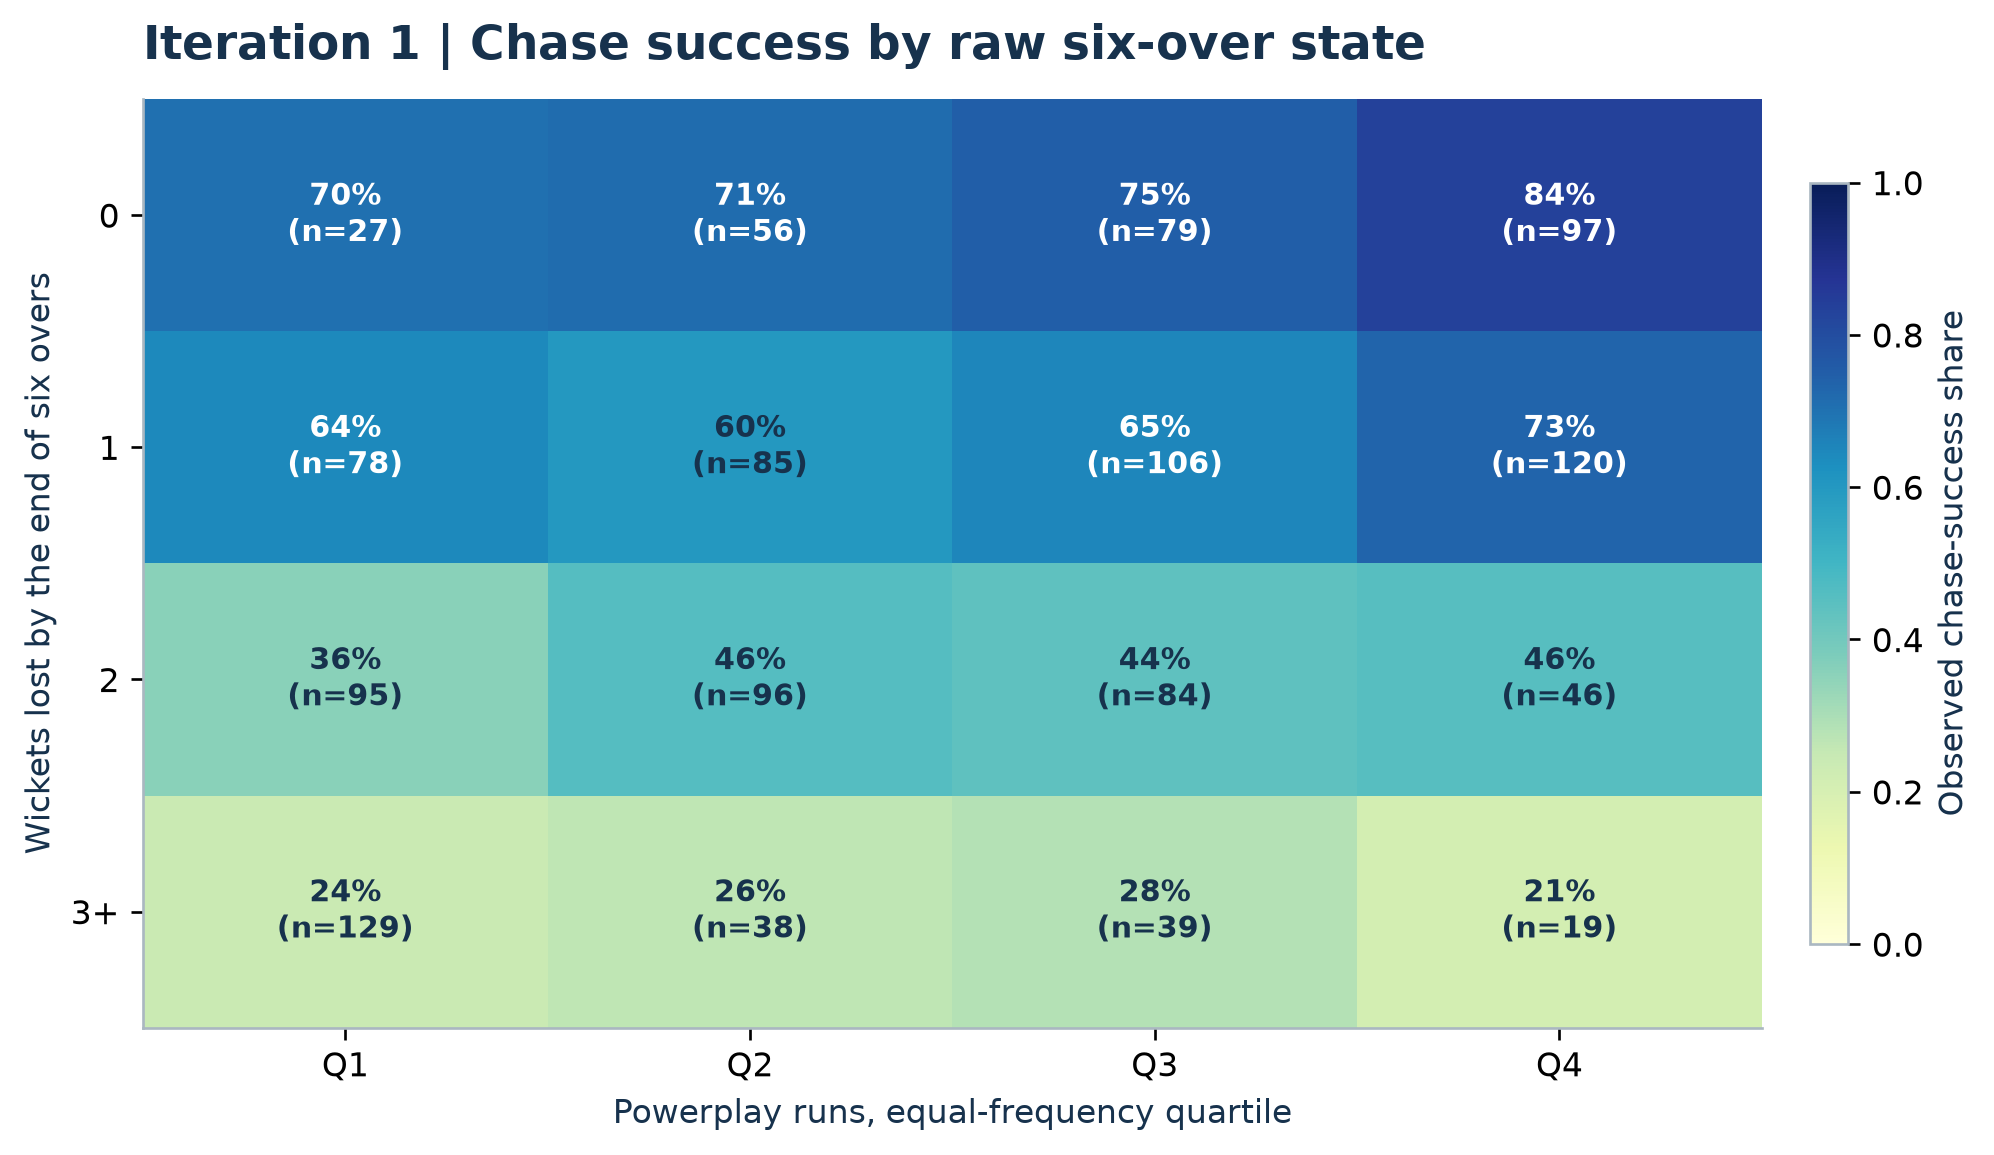
\includegraphics[width=0.83\linewidth]{iteration1_state_outcomes.png}
\caption{Iteration 1: chase-success share by powerplay run quartile and wickets lost. Cell labels show the observed share and match count. The matrix reveals how the two raw state variables relate to outcomes before target context is encoded.}
\label{fig:i1state}\end{figure}

\begin{figure}[H]\centering
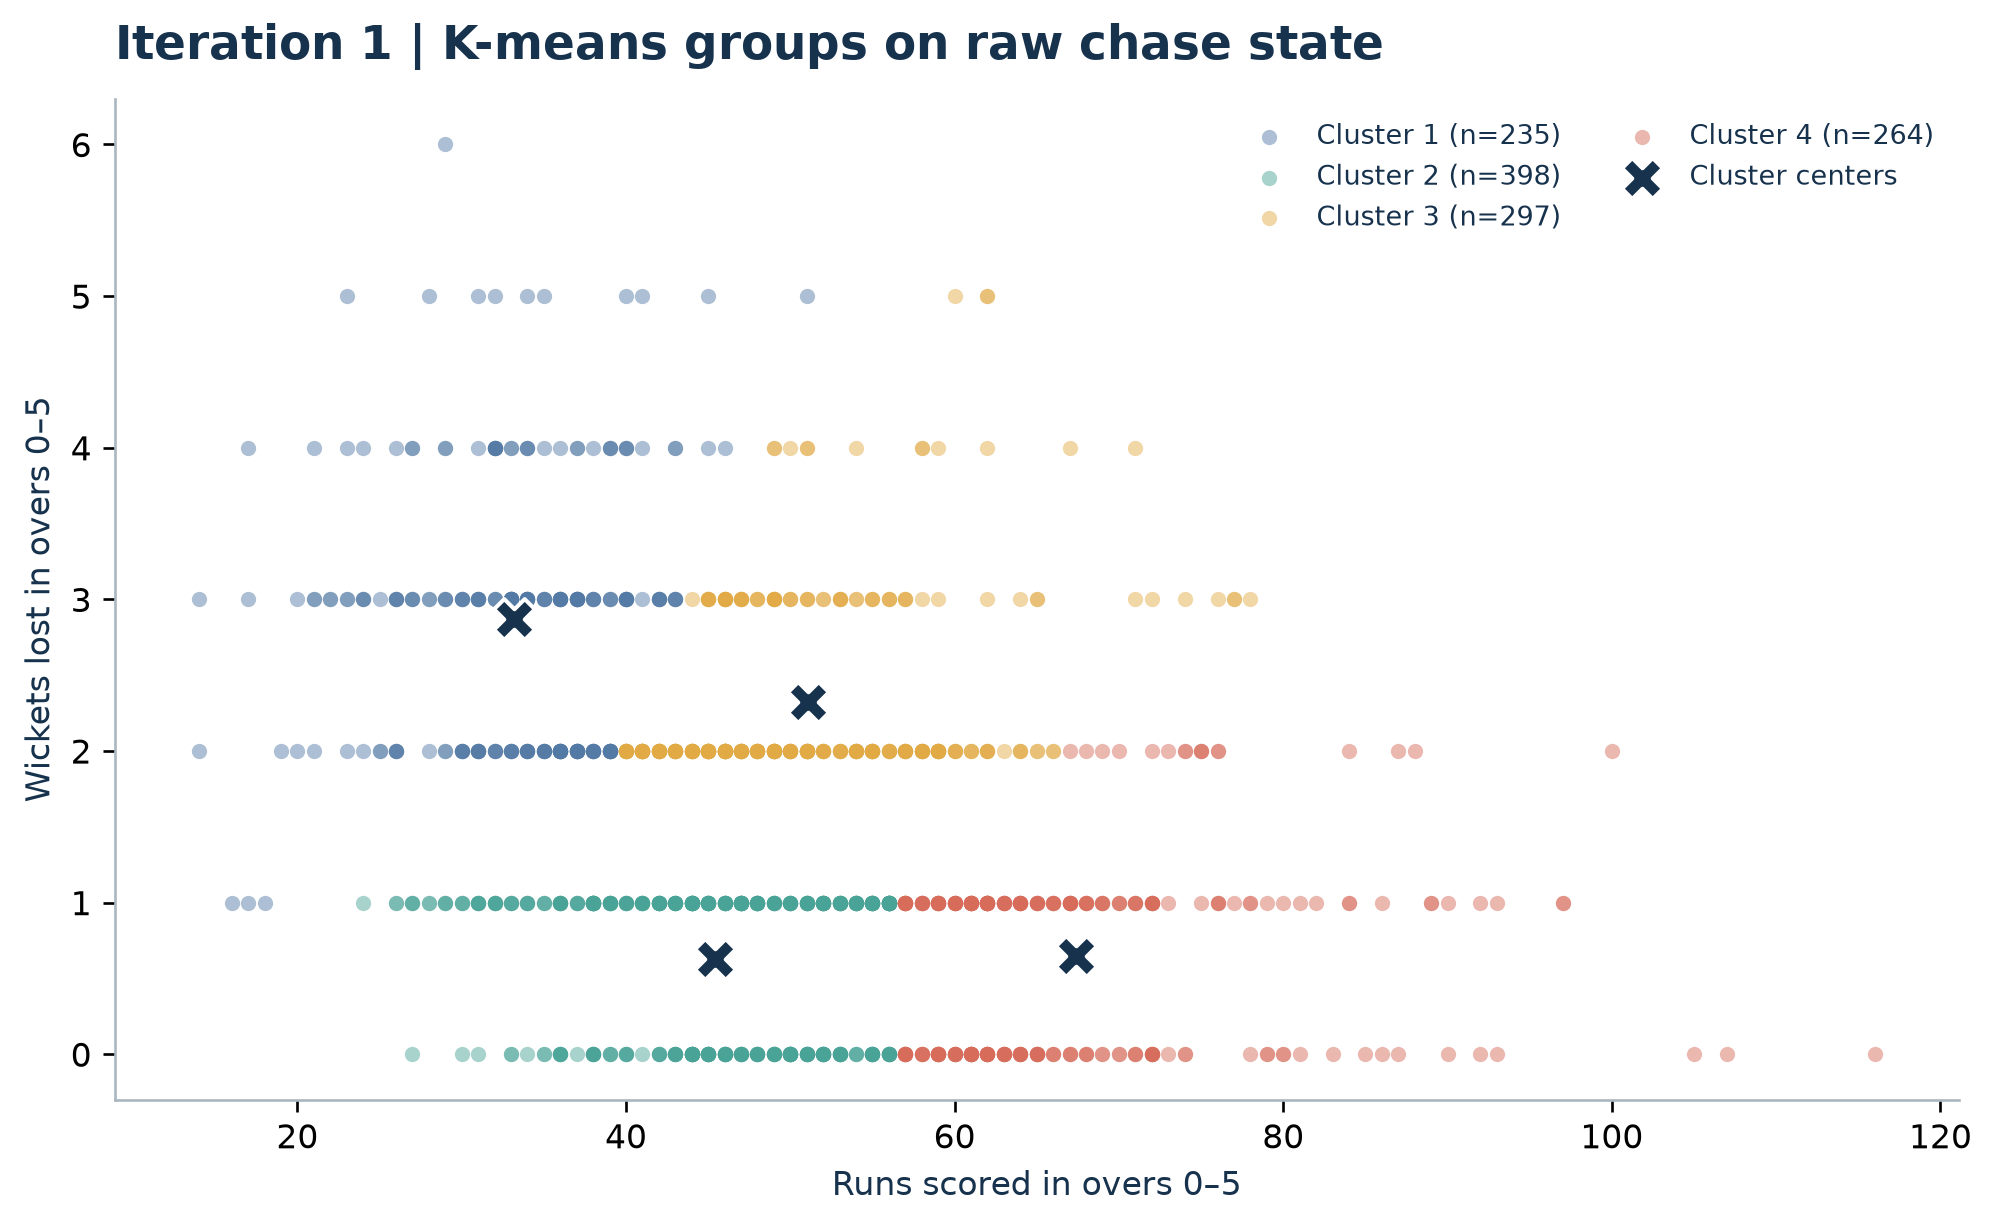
\includegraphics[width=0.82\linewidth]{iteration1_clusters.png}
\caption{Iteration 1 K-means projection. Points are match states; X markers are cluster centers. Cluster identifiers are display indices only.}
\label{fig:i1cluster}\end{figure}

\subsection{Iteration-one inference and feedback trigger}
The initial analysis suggested that score and wickets alone omit how much scoring remains necessary. The first-innings target is available before the chase, so required run rate at the checkpoint can be derived without using future deliveries. The lowest pressure quartile's success rate is 86.8\% and the highest's is 16.1\%, a Q1--Q4 difference of 70.7\% (95\% season-block interval 65.0\% to 76.3\%). This quantitative contrast justifies adding the number of runs remaining and required run rate to the state representation. It does not imply pressure caused the outcome.

\section{Feedback transformation}
The transformation adds \texttt{runs\_remaining = target - runs\_after\_six} and \texttt{required\_run\_rate = 6 * runs\_remaining / legal\_balls\_remaining}. Each row remains one match and keeps the same target, outcome, and raw six-over runs/wickets. No match is dropped by the transformation. The schedule's listed overs determine remaining legal balls. This changes the question from \emph{how much has the chase scored?} to \emph{how much must it score per over from here?}.

\section{Iteration 2: target-aware view}
Figure~\ref{fig:i2pressure} visualizes chase success by required-rate quartile with Wilson intervals. Figure~\ref{fig:i2cluster} repeats K-means after adding required rate, changing the clustering input from two raw state dimensions to a target-aware three-dimensional state. Figure~\ref{fig:models} compares the majority baseline and both logistic models on identical later-date matches.

\begin{figure}[H]\centering
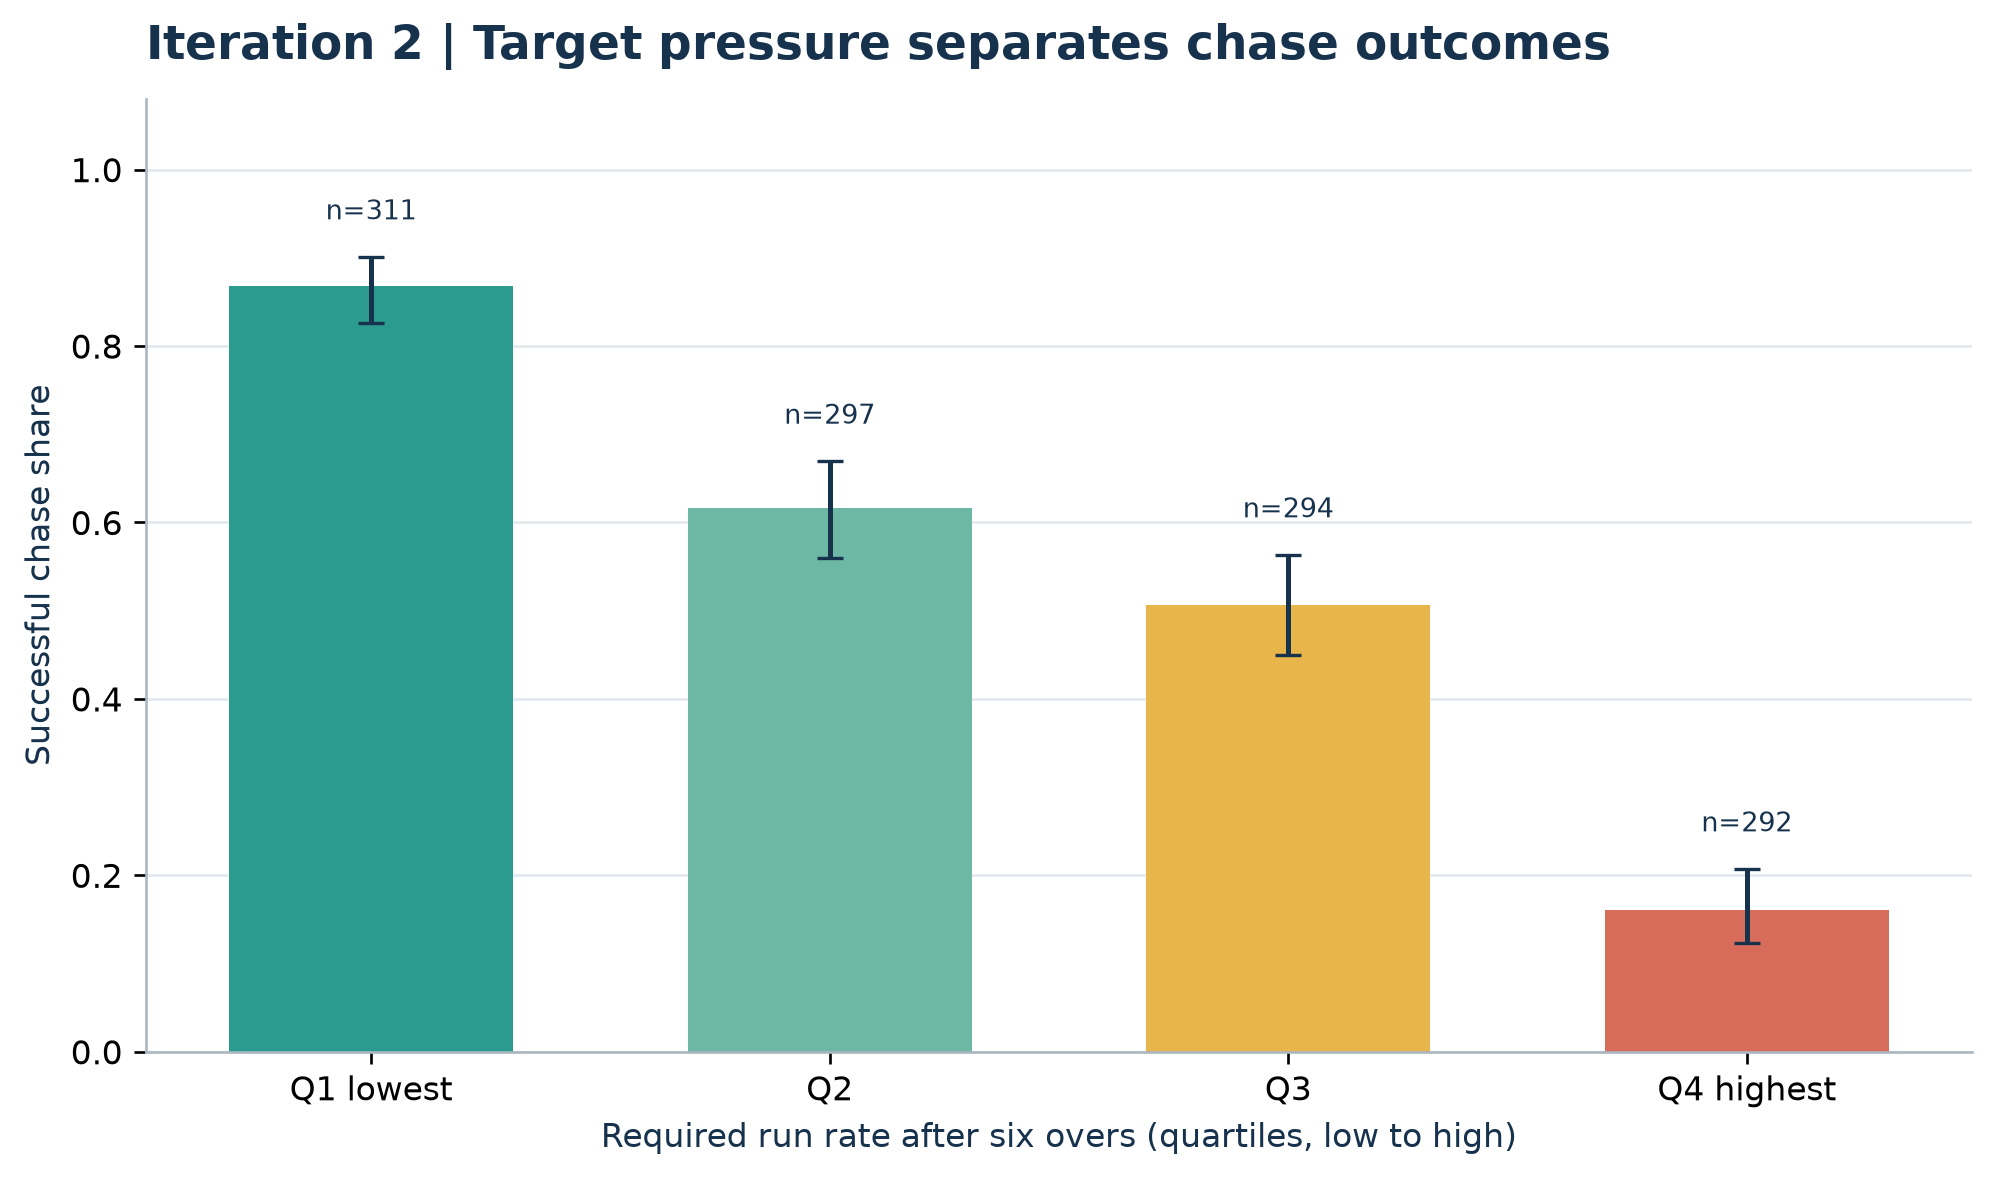
\includegraphics[width=0.83\linewidth]{iteration2_pressure_outcomes.png}
\caption{Iteration 2: observed chase success by required-rate quartile. Error bars are Wilson 95\% intervals; labels report sample sizes. The bootstrap interval in the text resamples season blocks.}
\label{fig:i2pressure}\end{figure}

\begin{figure}[H]\centering
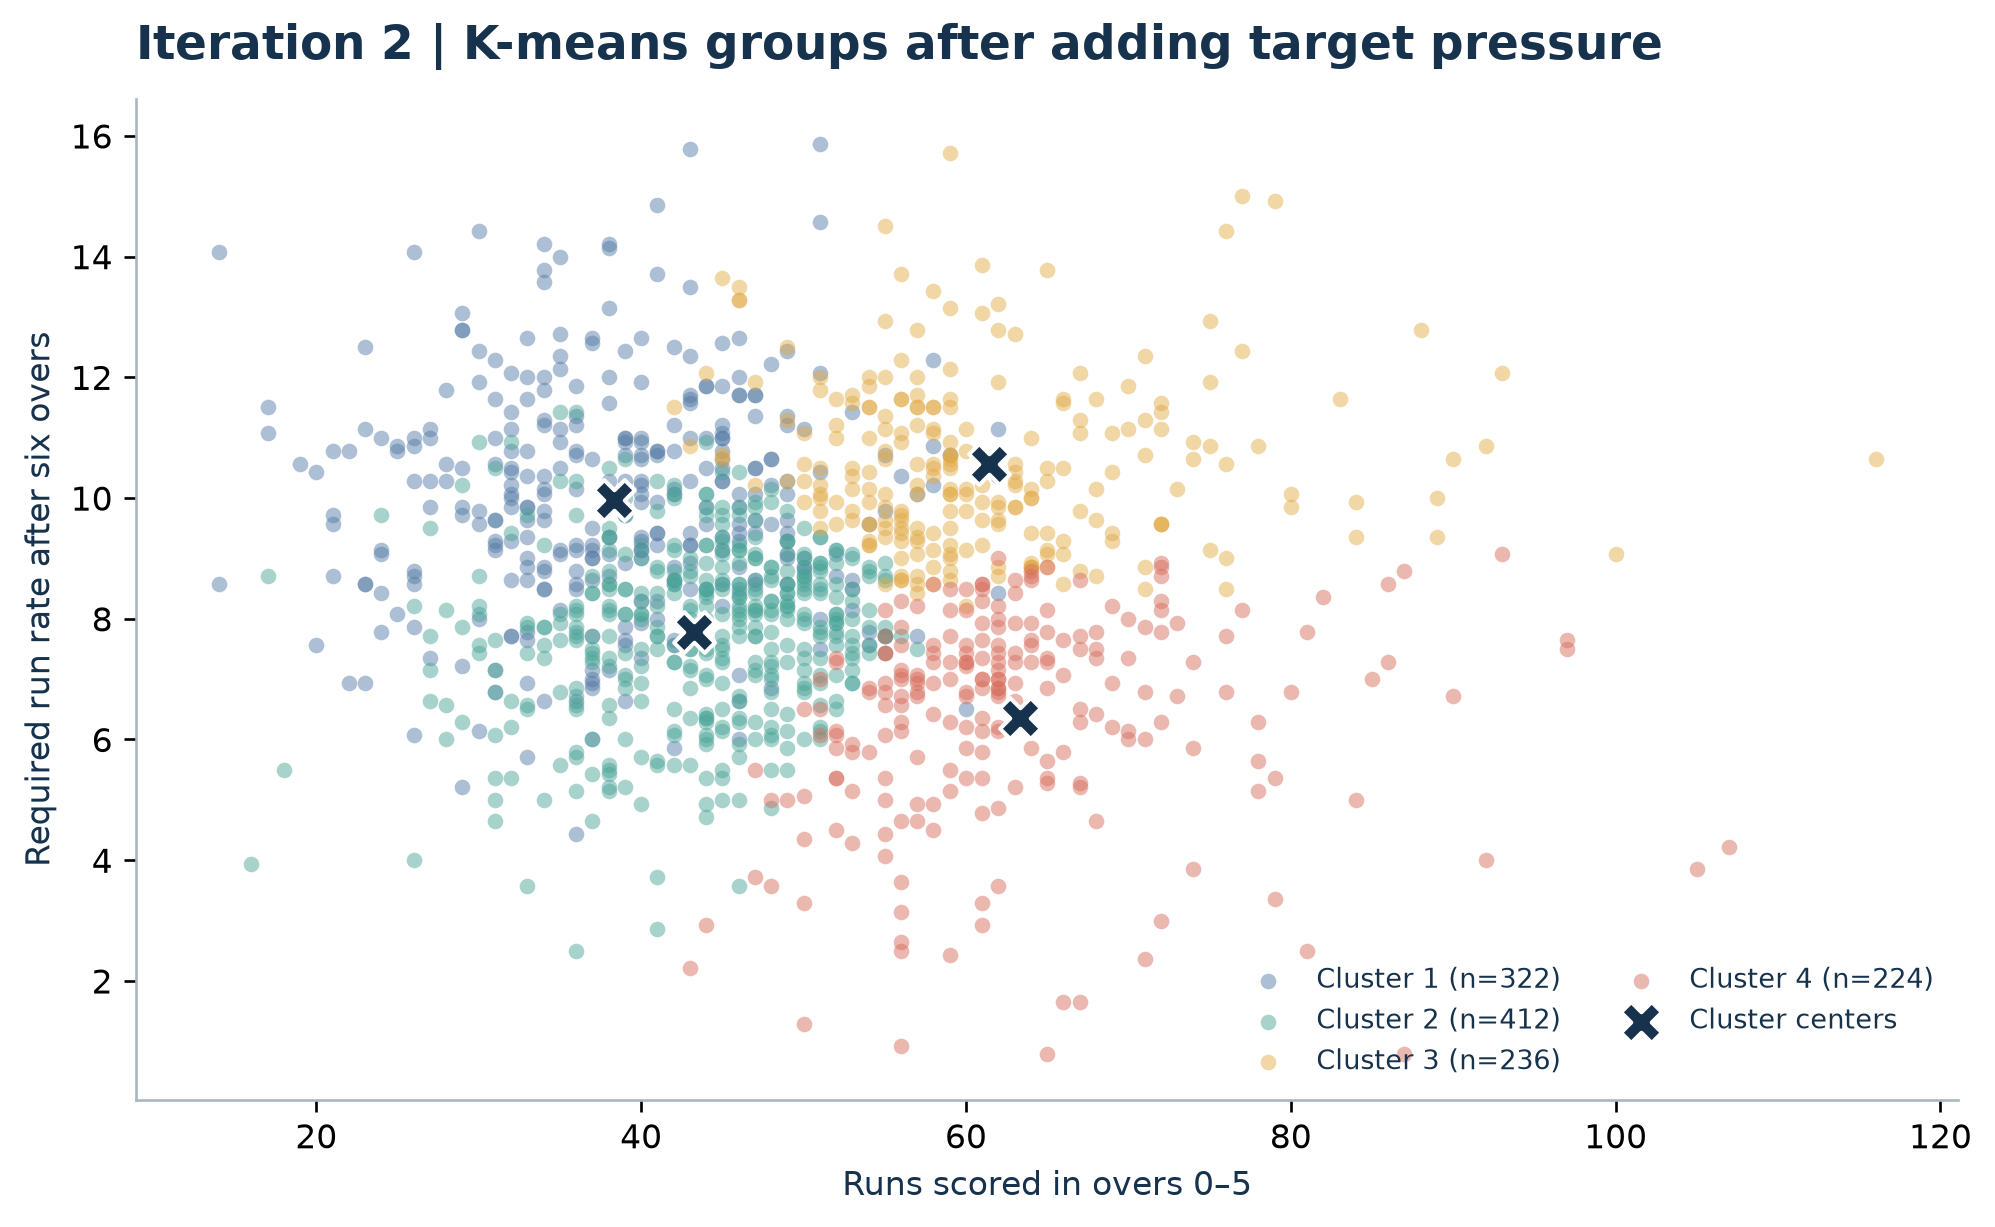
\includegraphics[width=0.82\linewidth]{iteration2_clusters.png}
\caption{Iteration 2 K-means projection after required run rate is added. The match rows are unchanged; this view displays how target context alters the represented state space.}
\label{fig:i2cluster}\end{figure}

\begin{figure}[H]\centering
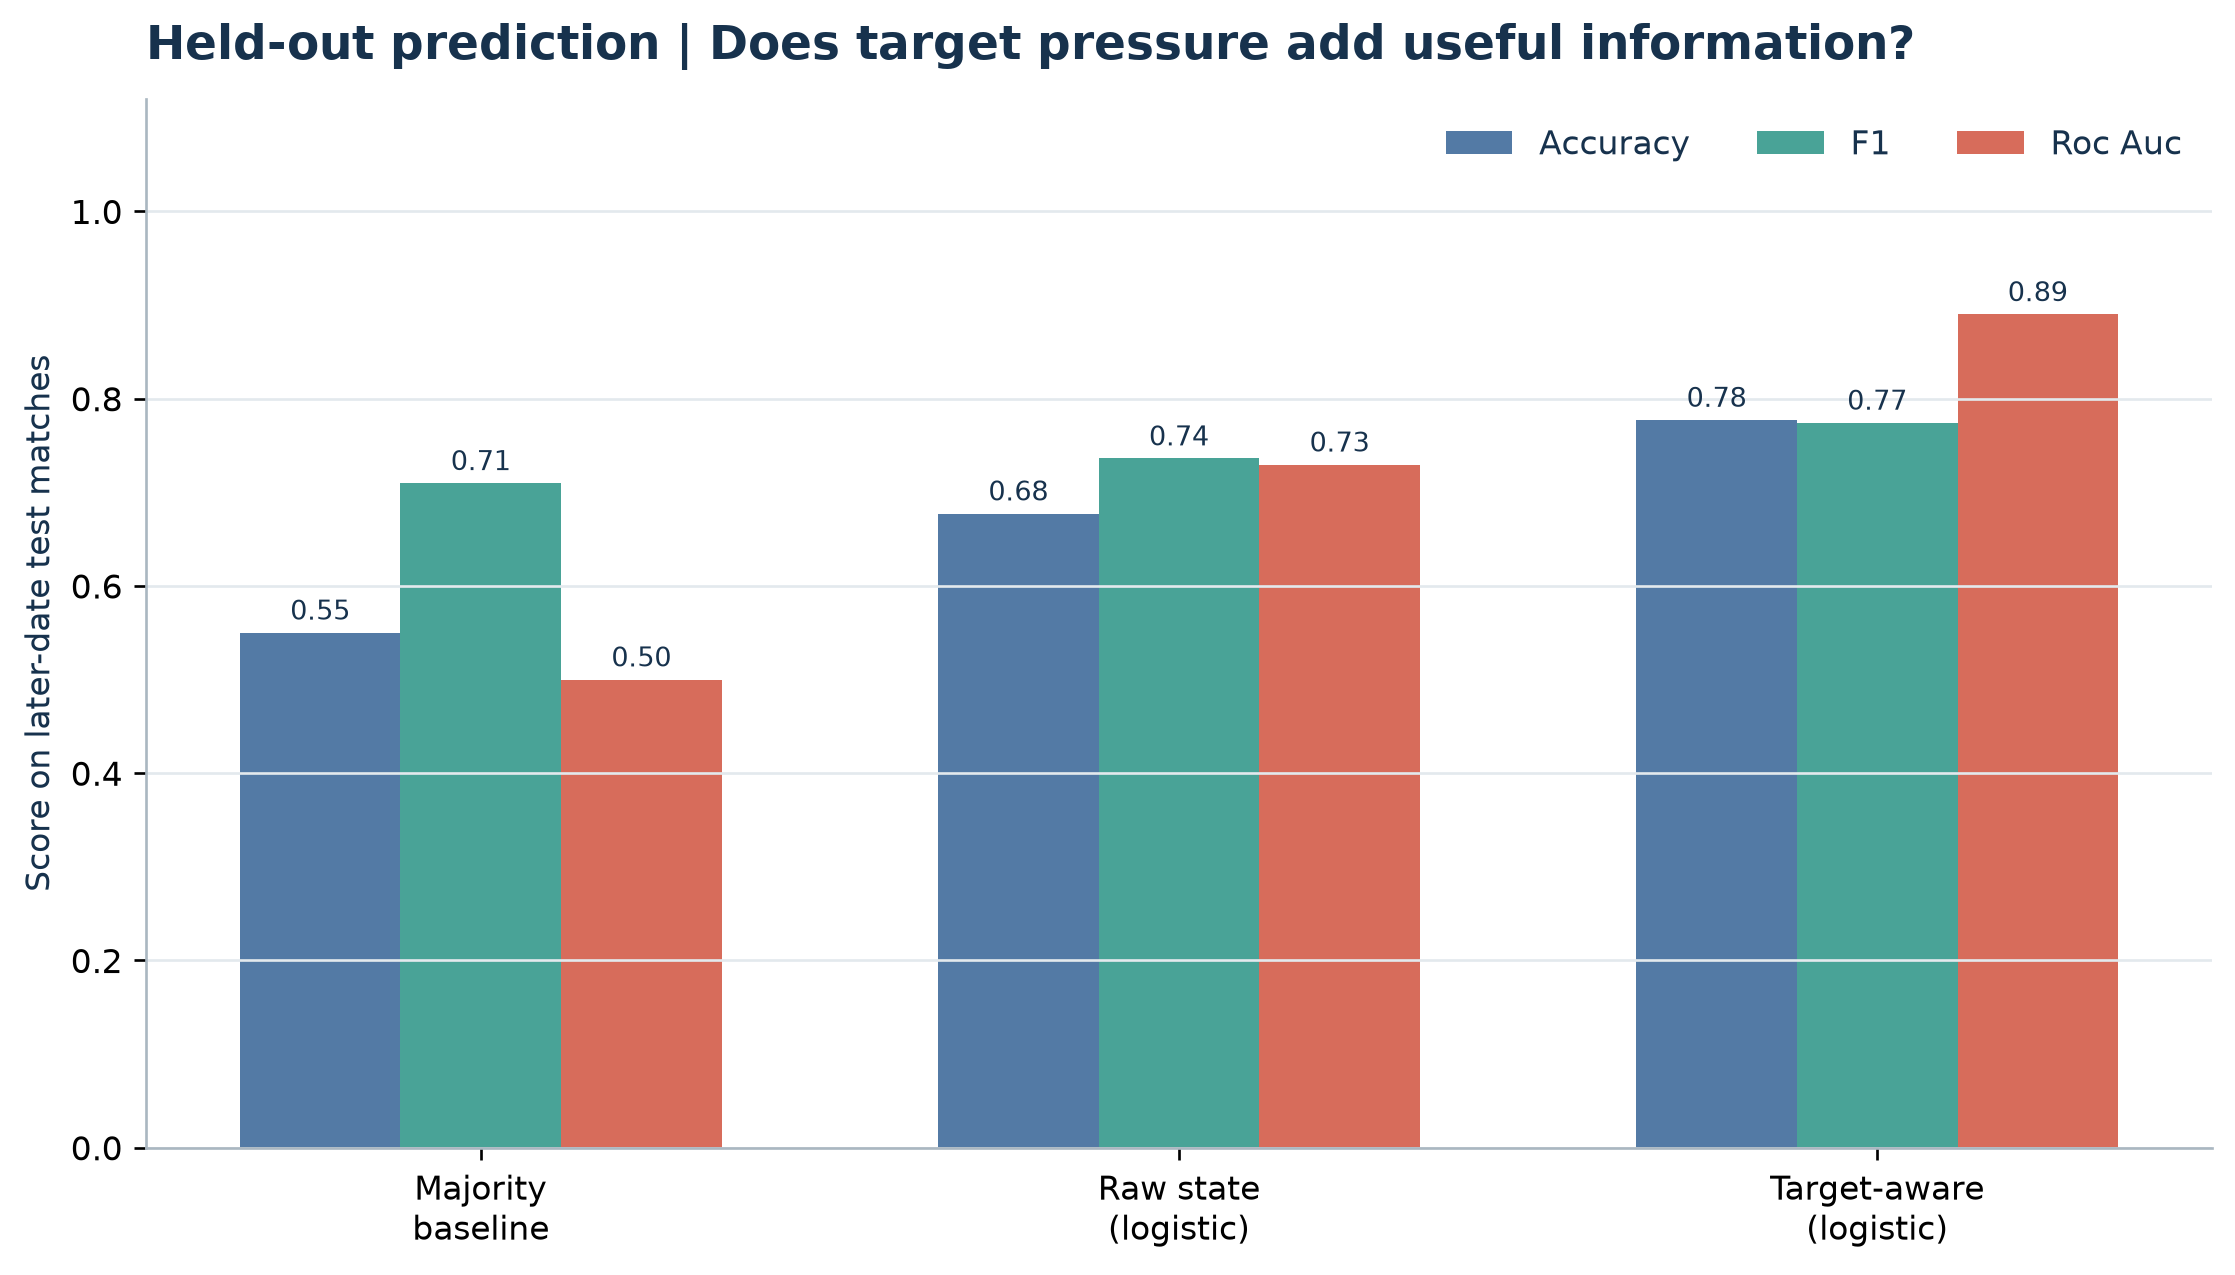
\includegraphics[width=0.86\linewidth]{model_comparison.png}
\caption{Majority baseline and logistic models evaluated on the same later-date holdout. Metrics are accuracy, F1, and ROC--AUC; higher is better.}
\label{fig:models}\end{figure}

On the chronological holdout, the raw-state model has accuracy 0.677, F1 0.736, and ROC--AUC 0.729; adding required rate gives accuracy 0.777, F1 0.774, and ROC--AUC 0.890. The majority-probability baseline has accuracy 0.550 and ROC--AUC 0.500. These results show whether the transformation improves prediction in this split; the Q1--Q4 descriptive gradient remains the main finding.

\section{Final findings}
\begin{enumerate}
\item Target-relative pressure distinguishes chase states that look similar when described only by six-over runs and wickets: the observed success share changes from 86.8\% in the lowest required-rate quartile to 16.1\% in the highest.
\item The transformed representation makes this relationship visible directly and lets the second logistic model test whether required rate adds held-out predictive information.
\item Clustering supplies a second view of state structure, but its labels are algorithm-dependent. It is not used to claim that cricket teams or chases fall into objectively discrete types.
\end{enumerate}

\section{Limitations and alternative explanations}
The data are observational. Team strength, opponent, toss, venue, rules, season, weather, and match conditions may influence both the six-over state and the outcome. A single chronological test period may differ from future seasons. The source contains repeated delivery rows and repeated over/ball keys; because identical wides may be distinct events and the available schema cannot disambiguate them, no blind deduplication was performed. Excluding D/L, short, tied, no-result, and early-ending chases narrows the population. The bootstrap uses only 19 season blocks. A future analysis could use over-by-over trajectories, season/team-adjusted models, calibration analysis, or a different target-normalized rate, provided that each feature is available at the prediction time and the test split remains valid.

\section{Conclusion}
The visual analytics workflow starts with raw six-over chase state, identifies a measurable omission, encodes that omission as required run rate, and returns to the data in a second visual and modeling iteration. The target-aware view answers a more useful question about progress relative to the task remaining. It provides an interpretable, reproducible story while keeping prediction separate from causal explanation.

\section{Team contribution statement}
\textbf{Placeholder -- complete with the group's agreed, truthful contributions before submission.} The A2 disclosure files list K V Shashank Pai, Adithya Kommuri, and Nishanth Karamsetty; confirm that this remains the A3 group. Add each member's actual A3 contribution. The technical workflow was implemented by the requesting student; confirm the name and describe only work that was actually performed.

\section*{References}
\begin{thebibliography}{9}
\bibitem{keim2008} D. A. Keim, J. Kohlhammer, G. Ellis, and F. Mansmann, editors, \emph{Mastering the Information Age: Solving Problems with Visual Analytics}. Eurographics Association, 2010. See also D. A. Keim et al., ``Visual Analytics: Definition, Process, and Challenges,'' in \emph{Information Visualization}, 2008.
\bibitem{macqueen1967} J. MacQueen, ``Some methods for classification and analysis of multivariate observations,'' in \emph{Proceedings of the Fifth Berkeley Symposium on Mathematical Statistics and Probability}, vol. 1, pp. 281--297, 1967.
\bibitem{hosmer2013} D. W. Hosmer, S. Lemeshow, and R. X. Sturdivant, \emph{Applied Logistic Regression}, 3rd ed. Wiley, 2013.
\bibitem{a3prompt} International Institute of Information Technology Bangalore, ``DAS732 Programming Assignment 3: Visual Analytics Workflow,'' Term 1 (2026--27), course handout.
\bibitem{a1report} DAS732 A1 IPL Analytics Project, ``IPL Cricket Data Story: A 15-Visualization Analysis,'' student report included in Appendix A.
\end{thebibliography}

\appendix
\section{A1 report (completeness appendix)}
The following pages reproduce the A1 report. As specified by the A3 assignment, this appendix is included for completeness and is not assessed as part of A3.
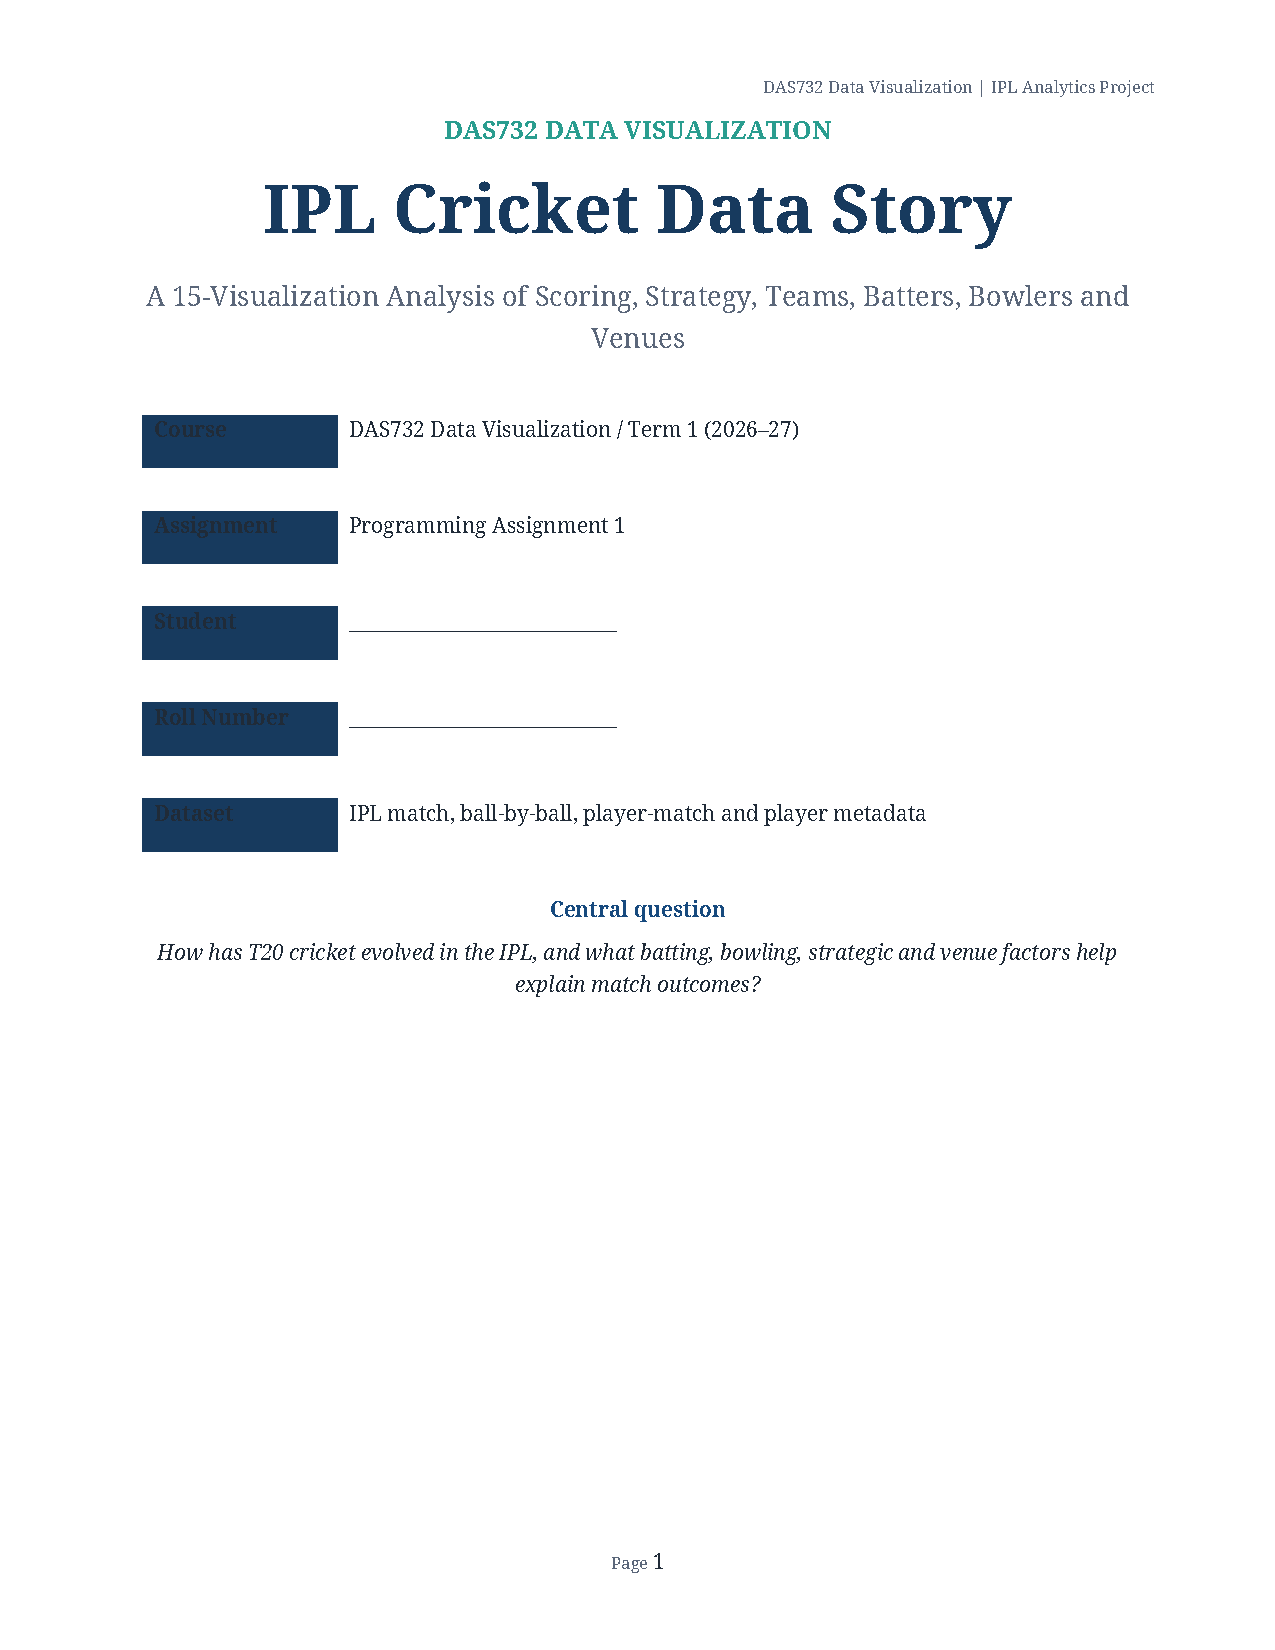
\includepdf[pages=-]{appendices/A1_Report.pdf}
\end{document}
